\subsubsection{$H \to \gamma\gamma$}
{\it To be written by: M. Delmastro}

\subsubsection{$H \to Z\gamma \to 2\ell\,\gamma$}
{\it To be written by: M. Delmastro}

\subsubsection{$H \to ZZ^* \to 4\ell$}
{\it To be written by: M. Delmastro}

\subsubsection{$H \to WW^* \to \ell\nu\,\ell\nu$}
{\it To be written by: M. Delmastro}

\subsubsection{$H \to \tau\tau$}
{\it To be written by: P. Francavilla, ?}

\subsubsection{$H \to bb$}
{\it To be written by: P. Francavilla, A. de Wit}

%% Macros from CMS
\newcommand{\TeV}{\ensuremath{\,\text{Te\hspace{-.08em}V}}\xspace}
\providecommand{\fbinv}{\mbox{\ensuremath{\,\text{fb}^\text{$-$1}}}\xspace}
\newcommand{\vh}{\ensuremath{\mathrm{V}\PH}\xspace}
\newcommand{\ttbar}{\ensuremath{\Pqt\Paqt}\xspace}
\newcommand{\zh}{\ensuremath{\PZ\PH}\xspace}
\newcommand{\ggZH}{\ensuremath{\Pg\Pg\PZ\PH}\xspace}
\providecommand{\wip}[1]{\textcolor{red}{\bfseries TODO: #1}\xspace}


\wip{Text currently reflects CMS studies only. Should be updated to reflect ATLAS and CMS studies.}

The ATLAS and CMS Collaborations have both reported the observation of the $\text{H}\to\text{bb}$ decay \cite{Aaboud:2018zhk,Sirunyan:2018kst}.
The studies presented here are performed based on a previous analysis, in which 
the CMS Collaboration reported evidence for the $\text{H}\to\text{bb}$ decay in the $\text{VH}$ production mode using the 2016
proton-proton collision dataset collected at $\sqrt{s} = 13\,\TeV$, which corresponds to an integrated luminosity of 35.9\fbinv \cite{HIG16044}. 
This analysis makes use of leptonic decays of the vector boson which is produced in association with the Higgs boson. The final states
of the $\vh$ system covered in this analysis always contain two b-jets and either zero, one or two electrons or muons. Both leptons are required to have the same flavour in the two lepton selection.
The b-jets are identified using a combined multivariate (CMVA) tagging algorithm. The inputs include track impact parameter and secondary vertex information from the jet. Three thresholds on the CMVA discriminant are used in the analysis, denoted tight, medium and loose, which have efficiencies for tagging b-jets ranging from $50$--$75\%$ and for light quark or gluon jets from $0.15$--$3\%$.

Major backgrounds arising from SM production of vector boson plus heavy- or light-flavour jets, in addition to \ttbar production, are 
controlled and constrained for each vector boson decay channel independently via dedicated control regions. Multivariate energy
regression techniques are used to improve the b-jet energy resolution, and a boosted decision tree is used to improve the discrimination 
between signal and background. The distribution of this multivariate discriminator is used as the discriminating
variable in the signal extraction fit. The signal strength observed in this analysis is 
$\mu_{\text{VHbb}} = 1.19^{+0.21}_{-0.20}\text{ (stat) }^{+0.34}_{-0.32}\text{ (syst) }$. Here the projected uncertainty
on the signal strength up to 3000\fbinv is reported, assuming $\mu_{\text{VHbb}} = 1$.

Figure \ref{fig:vhbb_projection_intlumi} shows the uncertainty on $\mu_{\text{VHbb}}$ as a function
of integrated luminosity, for scenario S1 (green points), scenario S2 (red points) and a scenario
where all systematic uncertainties are ignored (blue points).
In both scenarios
S1 and S2 systematic uncertainties start to dominate very quickly, thus moving the projected 
uncertainty away from the statistical-only scaling curve.

\begin{figure}[h!]
\begin{center}
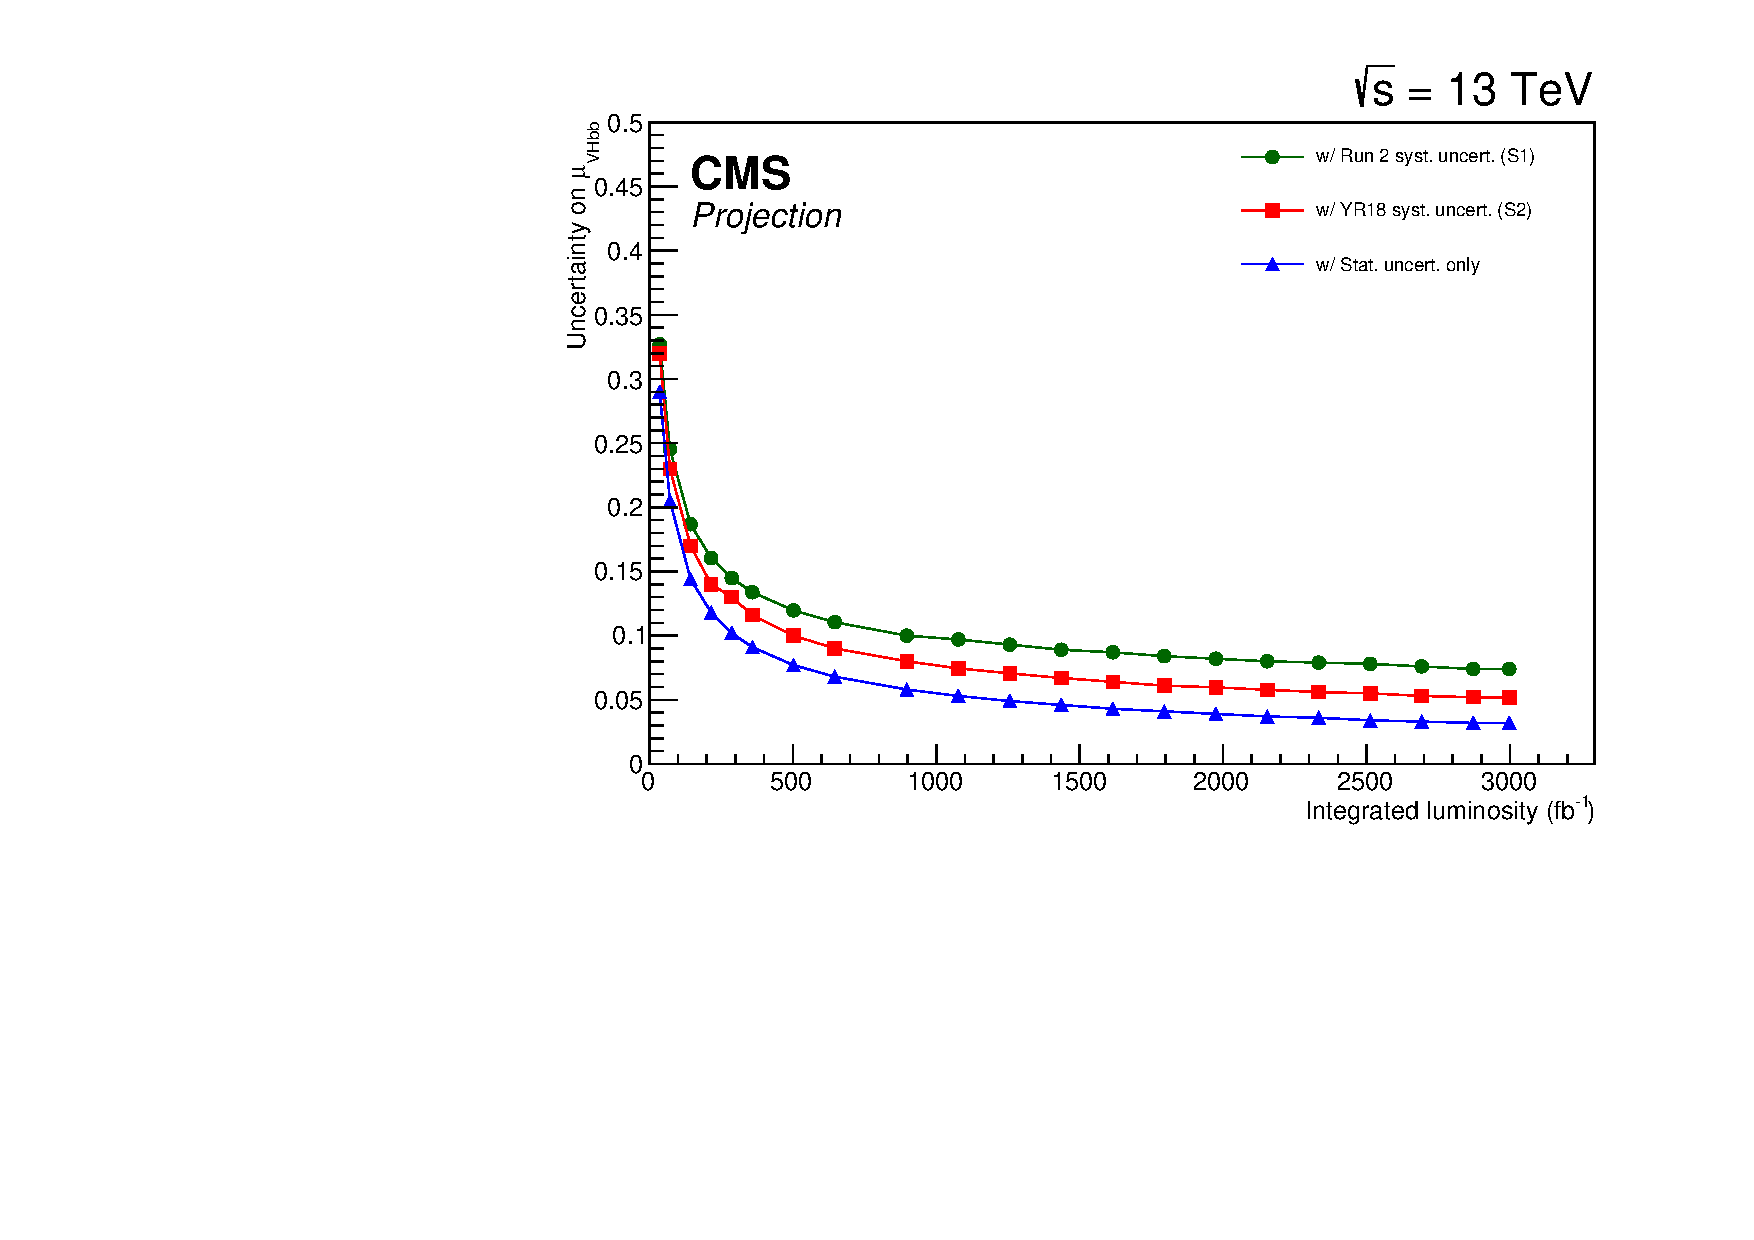
\includegraphics[width=0.75\textwidth]{\main/section2/plots/channels/vhbbprojection_mu_vs_lint.pdf}
\end{center}
\caption{Uncertainty on the signal strength $\mu_{\text{VHbb}}$ as a function of integrated luminosity for S1 (with Run~2 systematic uncertainties~\cite{HIG16044}) and S2 (with YR18 systematic uncertainties).}
\label{fig:vhbb_projection_intlumi}
\end{figure}

Figure \ref{fig:vhbb_proj_bars} shows the per-process and
per-channel signal strength uncertainty, showing results for all three scenarios described above.
The large improvement in the signal strength uncertainty for the 1-lepton channel, which is most sensitive to the WH production
mode, is caused by the integrated luminosity scaling of an uncertainty in the modelling of the $\PW$ boson $\pT$ distribution. This uncertainty dominates this channel
in scenario S1.

\begin{figure}[h!]
\begin{center}
% 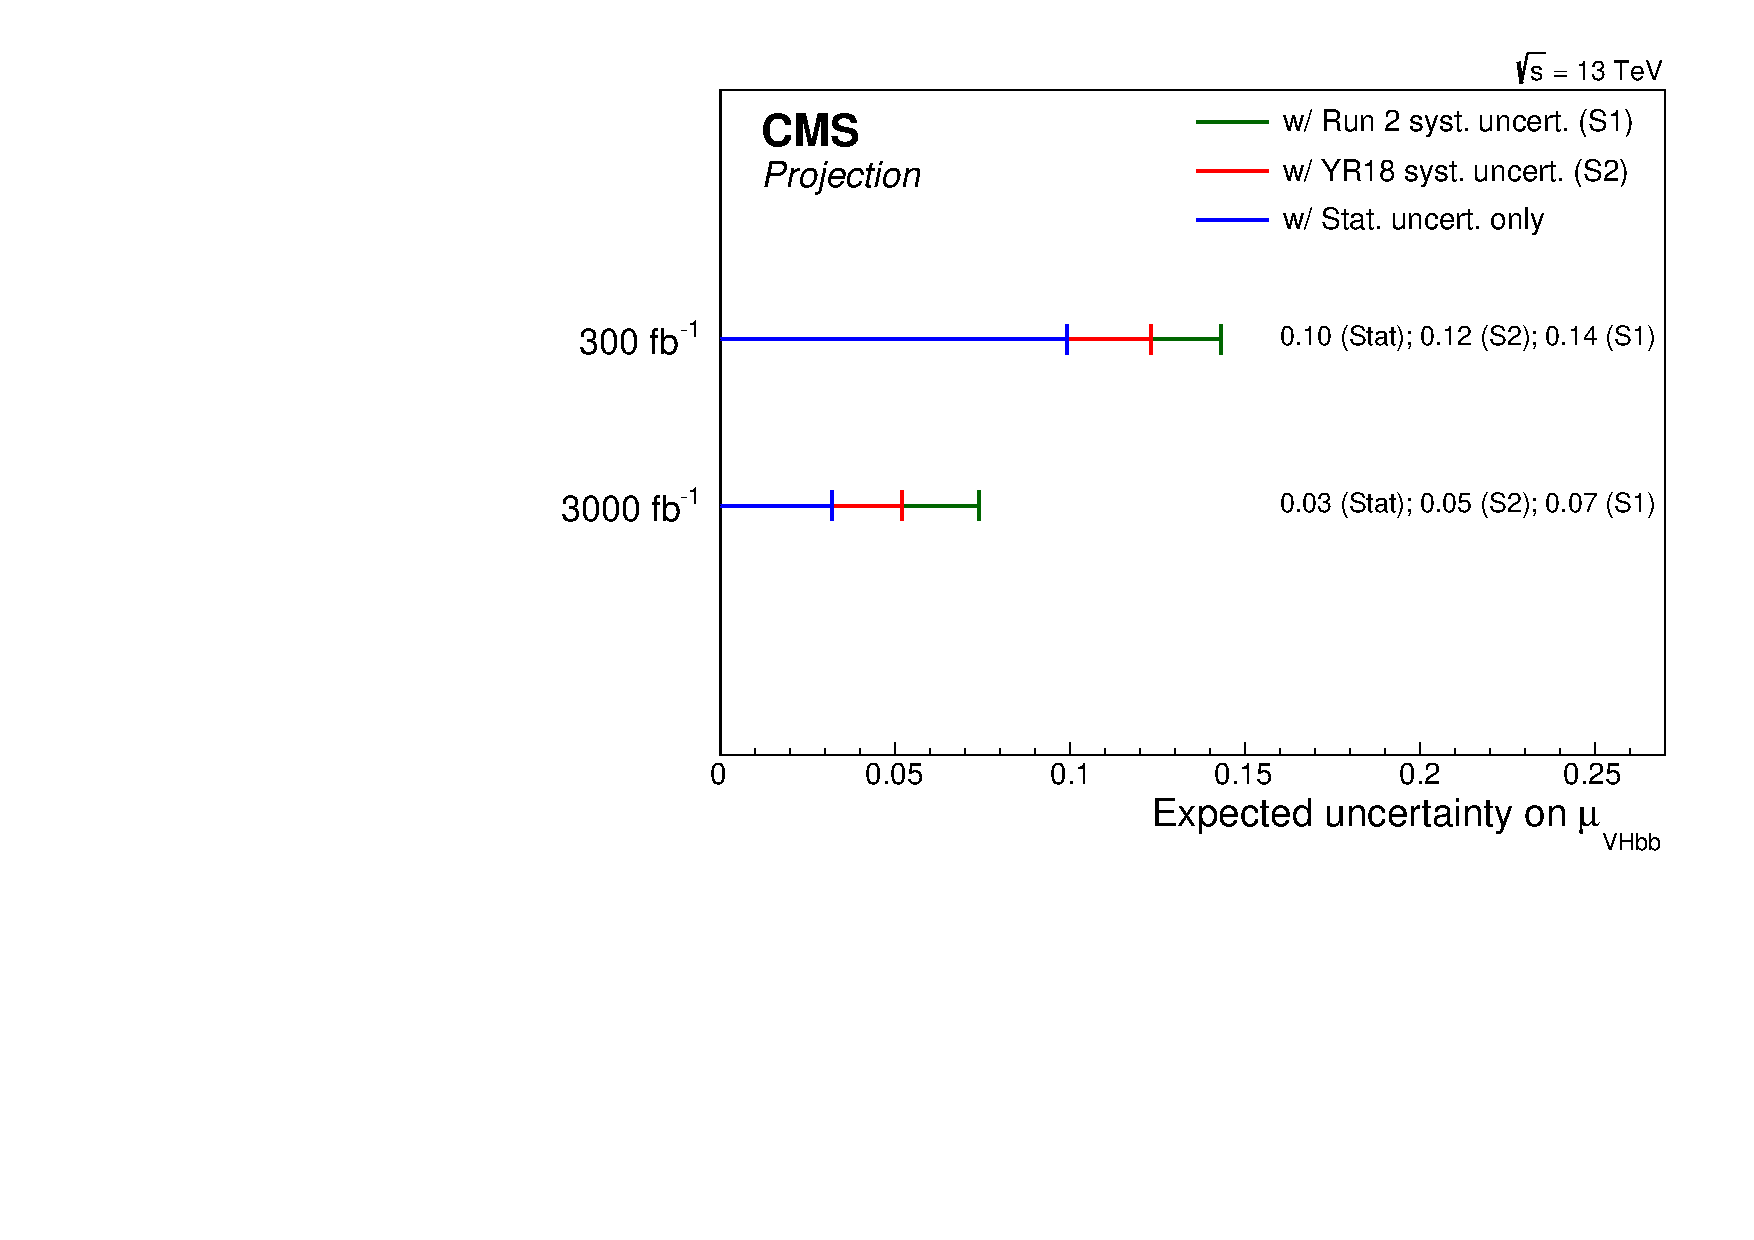
\includegraphics[width=0.48\textwidth]{\main/section2/plots/channels/Uncert300and3000.pdf}
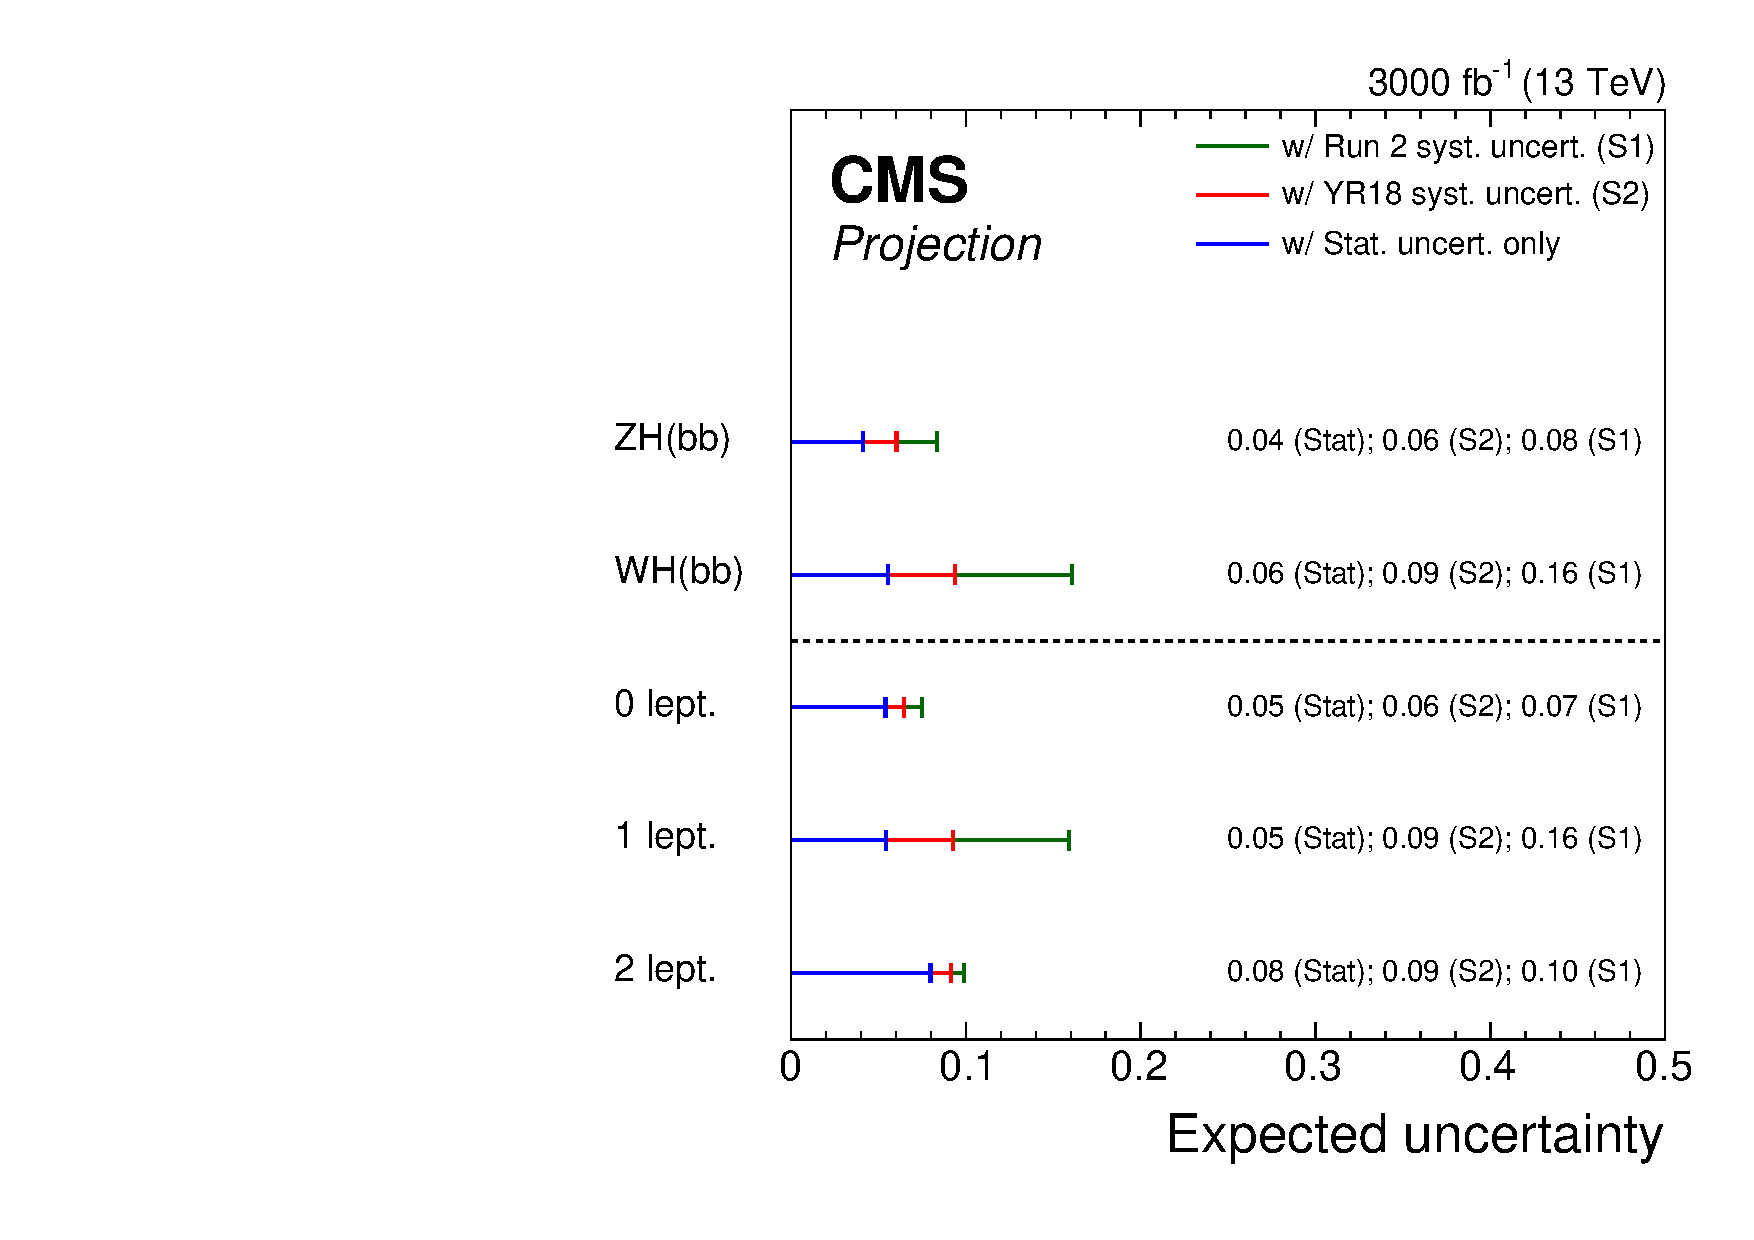
\includegraphics[width=0.6\textwidth]{\main/section2/plots/channels/ccc_3000fb_all.pdf}
\end{center}
\caption{Uncertainties in the per-process and per-channel signal strengths. Values are given for the S1 (with Run~2 systematic uncertainties~\cite{HIG16044}) and S2 (with YR18 systematic uncertainties) scenarios, as well as a scenario in which all systematic uncertainties are removed.}
\label{fig:vhbb_proj_bars}
\end{figure}

The contributions of different sources of uncertainty in scenarios S1 and S2 are shown in Table~\ref{tab:vhbb_uncertbreakdown}.
Both in scenario S1 and S2 the largest component of the systematic uncertainty is theoretical. Moving from S1 to S2 the total signal theoretical uncertainty reduces to half its size. This is expected as in scenario S2 the input uncertainties
are scaled down to half the current size. In the case of the background theory, where the input uncertainties are also scaled to half their original
size when going from scenario S1 to scenario S2, the total uncertainty due to this component is not halved. This is because at 3000 \fbinv
some of the theoretical uncertainties on the backgrounds can be constrained in the fit. The same is true for the experimental uncertainties, which
in some cases are already moderately constrained in the current analysis.

Looking in more detail at the dominant signal theoretical uncertainties, the largest component in the uncertainty arises from the uncertainty in the gluon-induced $\zh$ ($\ggZH$) production cross section due to QCD scale variations.
The $\ggZH$ process contributes a small fraction of the total $\zh$ process. Despite this, the uncertainty in the production cross section for this process due to QCD scale variations 
becomes dominant because it is very large: 25\% for the ggZH process, compared to approximately 4\% for the ZH process \cite{deFlorian:2016spz}.
The next most important uncertainties are category-acceptance uncertainties in the dominant Z+bb and W+bb backgrounds due to QCD scale variations, as well as the uncertainty in the ZH and WH production
cross section due to QCD scale variations. In scenario S2 these four most important uncertainties contribute 1.6\%, 1.5\%, 1.3\% and 1.2\% (absolute) to
the total uncertainty of 5.1\%, respectively. To improve the precision of the measurement it is therefore important to improve these theoretical uncertainties.

\begin{table}[th!]
\begin{center}
{
\caption{Contributions of particular groups of uncertainties in S1 (with Run~2 systematic uncertainties~\cite{HIG16044}) and S2 (with YR18 systematic uncertainties). The total uncertainty is decomposed into four components: signal theory, background theory, experimental and statistical. The signal theory uncertainty is further split into inclusive and acceptance parts, and the contributions of the b-tagging and JES/JER uncertainties to the experimental component are also given.}
\label{tab:vhbb_uncertbreakdown}
\begin{tabular}{l c c}
 & S1 & S2\\
Total uncertainty   & 0.073  & 0.051 \\
\hline
Signal theory uncertainty& 0.054 & 0.026\\
\quad Inclusive & 0.046 &0.022\\
\quad Acceptance & 0.027 &0.013\\
Background theory uncertainty & 0.028 & 0.023\\
Experimental uncertainty & 0.026 & 0.022 \\
\quad b-tagging & 0.022  & 0.020 \\
\quad JES and JER & 0.007  & 0.006 \\
Statistical uncertainty & 0.032 & 0.032\\
\end{tabular}
} % end footnotesize
\end{center}
\end{table}

In the future, and at the HL-LHC in particular, the b-tagging efficiency may change. The conditions could worsen the efficiency, but
at the same time new detectors and new techniques could also lead to an improvement in the b-tagging efficiency. 
The effect of changes in b-tagging efficiency on the overall signal strength uncertainty is evaluated. Changes in the b-tagging
efficiency are emulated by scaling the rates of processes with a single b-tag by the change in b-tagging efficiency, and scaling the 
rates of processes with two b-tags by the change in b-tagging efficiency squared. The modifications are applied only to the efficiency to select genuine b-jets; the mistagging rates for light quark and gluon jets remain unchanged.

Figure \ref{fig:vhbb_btageff} shows the results of the projection assuming various reductions and improvements in the b-tagging efficiency relative to the performance of the three CMVA working points used in the analysis.
A 10\% improvement in the b-tagging efficiency leads to a relative improvement in the signal strength uncertainty of up to 6\%. The improvements on the signal strength precision are limited because the uncertainty is dominated by theoretical sources. When neglecting inclusive signal theory uncertainties this improvement becomes up to 8\%. \wip{Results at $300\fbinv$ will be removed from the plot.}


\begin{figure}[h!]
\begin{center}
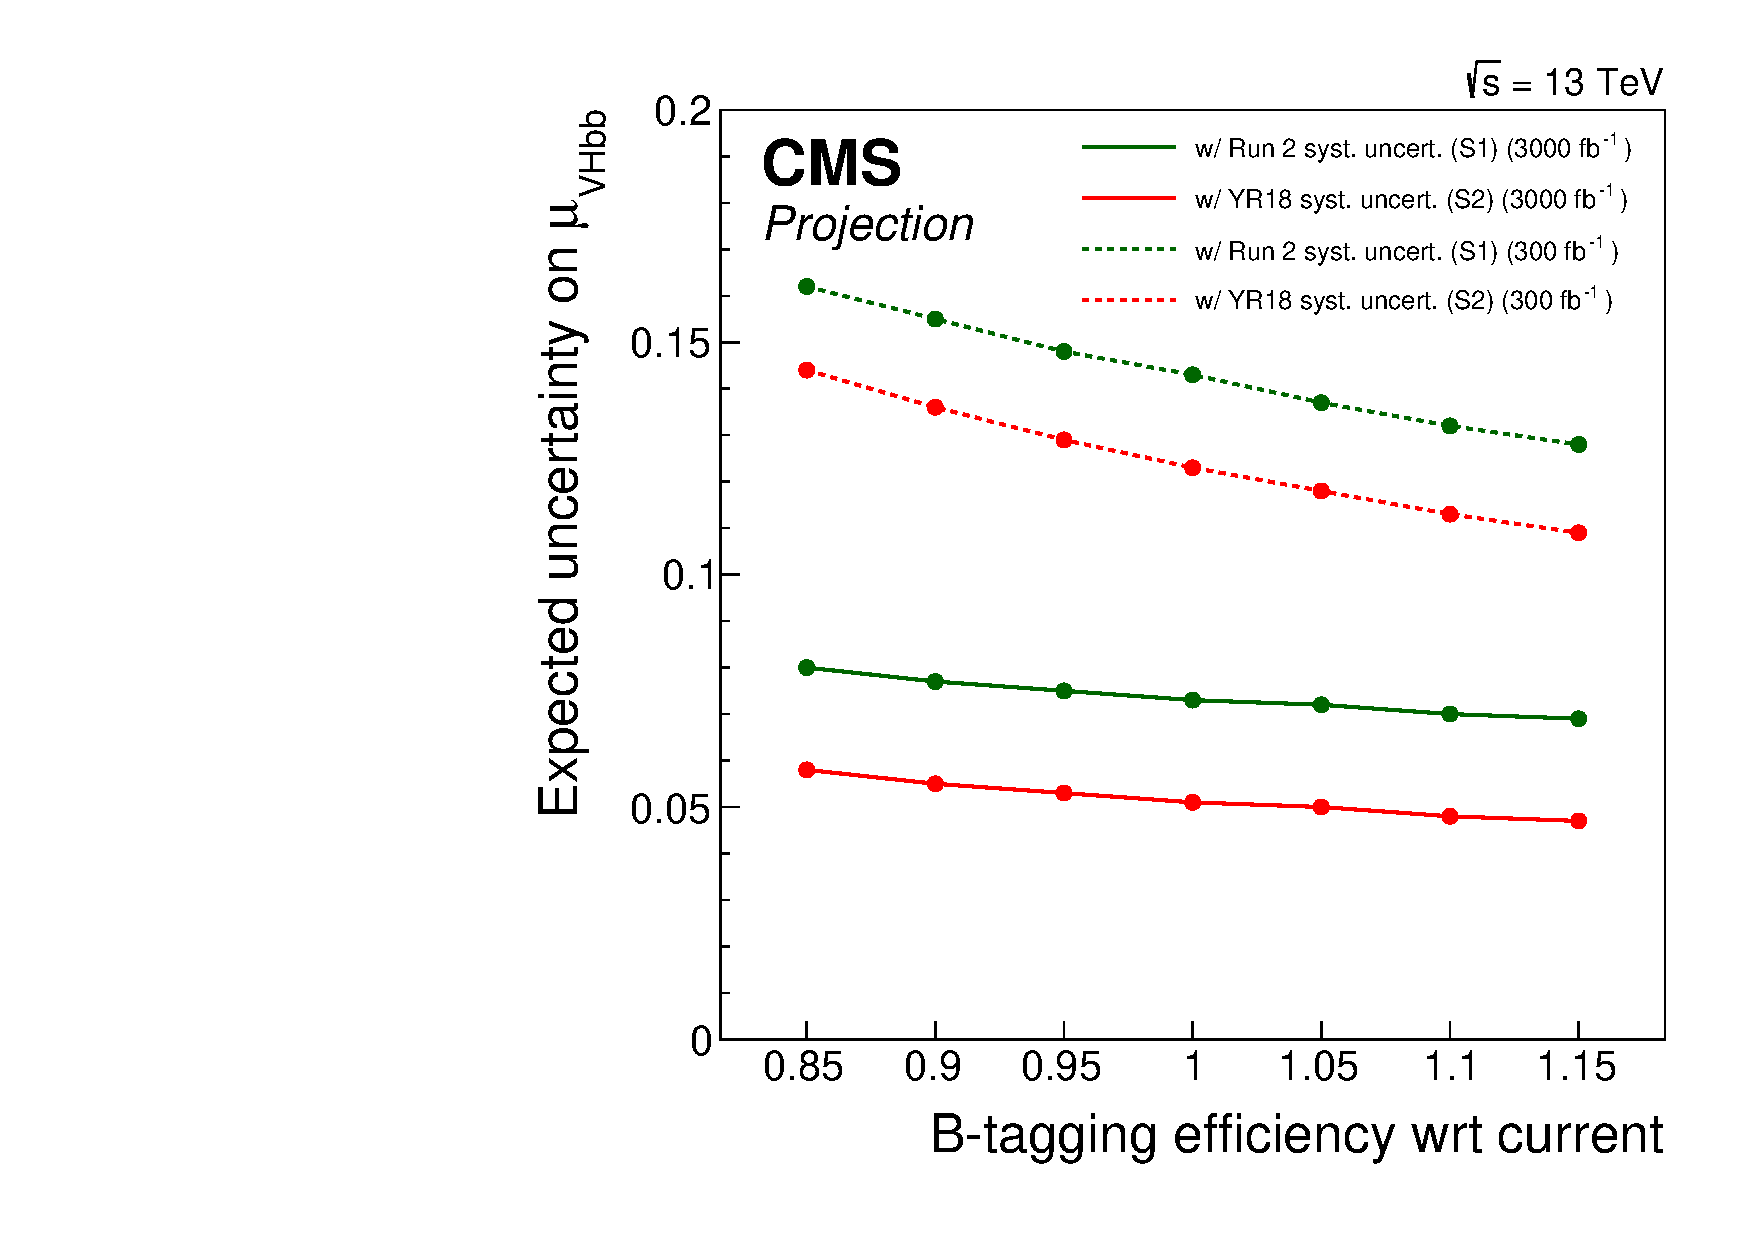
\includegraphics[width=0.5\textwidth]{\main/section2/plots/channels/BTagEff_Fig.pdf}
\end{center}
\caption{Effect of varying the b-tagging efficiency on the uncertainty in the signal strength measurement when considering all systematic uncertainties.}
\label{fig:vhbb_btageff}
\end{figure}

\subsubsection{$H \to \mu\mu$}
{\it To be written by: P. Francavilla, ?}
